\chapter{Probabilistic model}\label{chap:prob_model}
Since the proposed approach implements a probabilistic validation, the reliability of the result depends on the number of validators in the network in relation to the size of the iteration space. Given that the number of validators is finite, the probability of finding existing counterexamples may drop below an acceptable threshold for higher domain sizes. Thus, the distributed assertion checking scheme should provide a mechanism to have each validator invoke the assertion contract a specified number of times. To this end, it is necessary to identify a formula which, given the domain size and a probability threshold, returns a lower bound for the required number of test runs per validator. 

Sections \ref{sec:coupon} and \ref{sec:prob_threshold} describe the findings from a collaborative work with Julian Veigl \cite{bernhardt_veigel_2020}. They are based on the assumption that random generators pick elements independently from a uniform distribution. Furthermore, all calculations are based on the worst case scenario, in which there exists exactly one counterexample for the given input.

\section{Sample spaces}
The sample space of an assertion in form of a logical formula is given by the domains of discourse of the quantifiers. \secref described, that the premises defining the domains are translated into a list range constraints of the random generators. Based on these constraints, the compiler can derive a formula to determine the size of the sample space at runtime. In simple cases, the sample space is given by a single domain. Such a space is given, for instance, in the introductory example checking whether a number is a prime, i.e., $\mathcal{S} = \lbrace n \in\mathbb{Z} : 2 \le n \le \sqrt{p} \rbrace$. Based on the constraints $2 \le n$ and $n \le \sqrt{p}$, the size of the search space can be determined at runtime with $|\mathcal{S}| = \sqrt{p} - 2$. If the assertion has to sample from more than one domain, the search space is given by the Cartesian product of these domains, or sub-search spaces. In the example of intersecting sets from \secref{sec:existential}, the sample space is $\mathcal{S} = \mathcal{S}_U \times \mathcal{S}_V$, where $\mathcal{S}_U = \lbrace n \in\mathbb{Z} : 0 \leq n \le |U| \rbrace$ (analogue for $\mathcal{S}_V$). At runtime, the size of the search space can be determined with $|\mathcal{S}| = (|U| - 0) + (|V| - 0)$.

\section{Coupon Collector's Problem Analysis}\label{sec:coupon}
When checking properties with probabilistic testing, the result is either definitely not satisfied, or probably satisfied. Thus, errors only occur as false positives. In order to find a counterexample with probability $p = 1$, every element in the given search space $\mathcal{S}$ has to be checked by at least one validator. Deterministically, this is reachable with exactly $|\mathcal{S}|$ test runs. This is, however, invalid for the probabilistic approach, as some validators may generate duplicate random values and leave some elements of $\mathcal{S}$ unchecked. \\
In probability theory, this is known as the Coupon Collector's Problem \cite{croucher_collecting_2006}. Given $n = |\mathcal{S}|$, the probability that no duplicate elements are generated with $n$ picks is given by
\begin{equation*}
    p = \prod_{i=1}^{n} \frac{i}{n}
\end{equation*}
As an example, the probability that all validators generate a unique random value already drops to $0.036\%$ for $n = 10$. Let the random variable $T$ be the number of test runs executed until every element in the search space has been generated. In order to obtain an estimation of how many test runs are needed to find the counterexample for certain, the goal is to identify its expectation $E(T)$. To this end, the geometric probability distribution is applied \cite{croucher_collecting_2006}:\\
Each element is generated with a probability of $1/n$. Thus, the probability to generate the $i$th unique element is given by 
\begin{equation}
    p_i = \frac{n-i+1}{n}
\end{equation}
\cite{croucher_collecting_2006}. The expected value of a random variable $X$ is given by $E(X) = \frac{1}{p}$\cite{croucher_collecting_2006}, thus the expected number of test runs for $n$ is 
\begin{equation}
E(T) = n \sum_{i=1}^{n} \frac{1}{i}
\end{equation}
\tabref{tab:prob_outcomes} shows the expected number of test runs $E(T)$ and its standard deviation $\sigma$ for different $n$. Furthermore, $E(T)$ and $\sigma$ are used to calculate a 95\% confidence interval for $T$ by applying the central limit theorem, which provides an upper and lower bound on the number of test runs \cite{croucher_collecting_2006}. Rounded values for both bounds are also shown in \tabref{tab:prob_outcomes}.
\begin{table}[h]
    \centering
    \begin{tabular}{lllll}
        \thead{$n$} & \thead{$E(T)$} & \thead{$\sigma$} & \thead{lower bound} & \thead{upper bound}\\ \hline
        5 & 11.4 & 2.53 & 6 & 16\\
        10 & 29.3 & 4.32 & 21 & 38\\
        20 & 72.0 & 7.21 & 58 & 86\\
        30 & 119.8 & 9.48 & 101 & 138 \\
        50 & 225.0 & 13.23 & 199 & 251 
    \end{tabular}
    \caption{Expectation, standard deviation and upper and lower bound of needed test runs for some $n$ \cite{croucher_collecting_2006}}
    \label{tab:prob_outcomes}
\end{table}

The results show that checking random values is a very inefficient approach if false positives are not admissible. Even if the lower bound of $T$ is chosen as the number of test runs, it exceeds the size of the search space by far and increases the time complexity to $\mathcal{O}(n*log(n))$ for large $n$ \cite{xu_tang_2011}. For instances where false positives are tolerable, the following section introduces a formula to calculate the number of test runs that detect counterexamples with a given probability threshold $p \leq 1$.

\section{Setting probability thresholds}\label{sec:prob_threshold}
The goal is to find a number $t$ of test runs, s.t. the probability $P_{c,t}$ of not finding the counterexample drops below a certain threshold $c$. A validator finds the counterexample in one test run with probability $\frac{1}{n}$, and misses it with probability $(1-\frac{1}{n})$. After $t$ tests runs, the probability that the counterexample has not been found is thus $(1-\frac{1}{n})^t$. Following the same approach as in \cite{mahl_schindel_2007} to retrieve an upper bound for $P_{c,t}$, we use the following inequality
\begin{equation}
(1-\frac{1}{m})^m \leq \frac{1}{e}
\end{equation}
which holds for all $m > 0$. From this inequality, it follows that
\begin{equation}
(1-\frac{1}{n})^t = ((1-\frac{1}{n})^n)^{\frac{t}{n}} \le e^{-\frac{t}{n}}
\end{equation}
With this, the probability $P_{c,t}$ of not finding the counterexample with $t$ test runs can be defined as
\begin{equation}
P_{c,t} \le e^{-\frac{t}{n}}
\end{equation}
In order to retrieve the number of test runs $t$ necessary for $P_{c,t}$ to drop below a specified threshold $c$, the inequality is solved for $t$, which is then dependent of the known parameter $n$ and an arbitrary value for $c$:
\begin{align}
    e^{-\frac{t}{n}} &\leq c && \text{with } 0 \leq c\le 1 \nonumber\\
    t &\geq -n\:\ln(c)
\end{align}
For $c = \frac{1}{e}$ ($\approx 36.79\:\%$) the lower bound of $t$ is exactly $n$, which means that for higher reliabilities the number of test runs needs to be greater than $n$. \figref{fig:graph_t_c} shows the lower bounds of $t$ as a function of the probability threshold and search space size. One can see that the increase in accuracy is approximately linear to the number of test runs below a threshold of $c=0.5$, but requires an exponential testing effort to reach higher thresholds.
\begin{figure}[h]
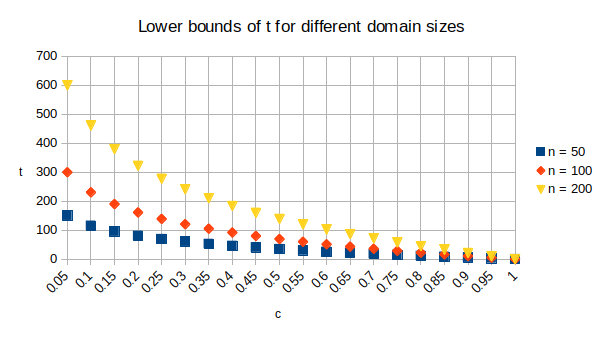
\includegraphics[width=0.95\linewidth]{figures/3-offline/graph_t_c}
\caption{The number of required test runs as a function of the probability of false positives $c$ and size of the search space $n$}
\label{fig:graph_t_c}
\end{figure}

\section{Validators vs. test runs}
The last section derived a formula to calculate a lower bound for a number of test runs $t$ in order to reach a certain level of confidence. However, $t$ is not a parameter that can be adjusted to an arbitrary value on the blockchain, as the assertion is checked by the validators. Assuming a blockchain has $m$ validators, the actual lower bound of test runs is $m$. For cases where there are not enough validators to reach a threshold $c$, a mechanism is required to have each validator check the property for multiple random values. Hence, the actual executed number of checks is always a multiple of $m$.

\section{Alternatives to random testing}\label{sec:alt_random}
For applications where higher reliability is crucial, an alternative to checking elements randomly could be to coordinate a systematic iteration of the domain. The implementation of such a coordination is not trivial though; validators can't simply be passed an individual value as input. Instead, possible approaches could be to implement a central instance that allocates an element in the search space to each validator, or use some unique and intrinsic attribute, like an identification number, as input for a mapping.

\subsection{Central instance assigning values}
For this approach, the tool-chain would need to generate a separate contract that is called by the miners and validators as a proxy. This contract would then, for instance, generate a number using a modulo-n counter and pass this number as an additional parameter to the assertion code. The random generators would be omitted accordingly. However, this works only as expected if there are no simultaneous transactions calling the contract, otherwise it cannot be guaranteed that all elements have been checked for each of the transactions. If and how this issue can be solved will not be discussed further in this thesis. Another drawback of this approach is that it leads to a serialization of the tests, as the contract has to update its internal storage.

\subsection{Using unique attributes of a validator}\label{sec:alt_attributes}
This approach strongly depends on whether the validators have a unique id or other attribute that can be accessed from within a contract.  If there is (or the language can be extended with such a feature), there needs to exist a non-injective surjective function that maps the respective attributes represented by type A to an element in the search space, represented by type B, i.e. $f: X \rightarrow Y$. Furthermore, for cases where $t > m$, an offset needs to be added, s.t. a validator checks distinct elements for each test run. \\
Implementing such an approach on Tezos becomes even more challenging due the way endorsing (i.e. validation) rights are distributed in its proof-of-stake mechanism: for each block level, endorsing rights are assigned to the owner of a randomly selected roll, i.e., a set of tokens \cite{tezos_docs}. This means that the same validator can be picked multiple times for endorsing one block and thus some elements in the search space may remain unchecked. \secref{} goes into more detail about this issue. \todo{Ref section}